\section{Insa Suchantke}
\textbf{Responsibility: App development, Design decisions}\\
\textbf{Role: Organisation Master}\\

\subsection{Available smartphone apps in palliative care}
There are not many smartphone apps for palliative care on the market \cite{nwosu}. One of these apps is \textit{Alberta}\footnote{https://halloalberta.de} which is a care management platform for chronically ill patients to manage the entire patient care digitally. It has various features like digital documentation, appointment and route planning and complete patient files with all patient-related data. Another app is \textit{PalliDoc}\footnote{https://www.pallidoc.de} which is a software for palliative care. It offers for example team-specific overviews, task management, care documentation, symptom recording and determination of travel routes.
With the \textit{biotronik}\footnote{https://www.biotronik.com/en-de/patients/patientapp} app the cardiac status of patients with an implanted BIOTRONIK cardiac monitor BIOMONITOR III can be measured. In this app there also exists a diary function of the symptoms. \textit{Myo}\footnote{https://myo.de} app is a platform for communication between caregivers and relatives. The app \textit{vivifyhealth}\footnote{https://www.vivifyhealth.com} offers a remote patient monitoring platform for chronic and post-acute care with for example informative content for the patients and monitoring the biometric data of the patient.

Furthermore, there are also smartphone apps that provide information and facts about palliative care, such as \textit{Palliative Care Fast Facts}, \textit{Pocketbook of Palliative Medicine}, \textit{NHS Palliative Care Guidelines} and \textit{Palliative Care ACT}.

The Alberta and PalliDoc apps are the only ones that offer patient management. Only \textit{biotronics} and \textit{vivifyhealth} provide an integration of medical devices. \textit{PalliDoc}, \textit{myo} and \textit{vivifyhealth} have an interface for the care team and the doctor. An interface also for nok is just available at \textit{myo}. The apps \textit{biotronik} and \textit{vivifyhealth} make it possible to monitor the patients' state of health. 

Although all these apps provide nice features like patient management, integration of medical devices, interfaces for doctor, care teams or nok and monitoring the patients‘ state of health, no app combines the shared accessibility for patient, nok and SAPC team with data analysis and health status monitoring of the patient. Such an interdisciplinary platform must exist so that patients can be cared for at home and be enabled to die with care.

\subsection{PalliCare Smarthpone App - Design and layout decisions}
Most of the palliative patients have ages between 70 and 79 years with an average age of 70 \cite{rki1}. Because of that the layout of the \textit{PalliCare} smartphone app had to be adapted to the high average age of these patients. In order to get a feeling what kind of layout and design is appropriate for older people, it has been examined which apps are already on the market for this age category.   

One of these apps is the \textit{SwissVoice CS50s}\footnote{https://www.swissvoice.net/de/produkt/c50s-0} smartphone, which has adapted features and layout for older people. For example, the ringtone and volume can be adjusted to an extra loud level and has further large icons to aid comprehensibility. The smartphone app \textit{Koala Phone Launcher Free}\footnote{https://tomas-slavicek-koala-phone.de.aptoide.com} is intended for older people who use the smartphone for the first time and also for those who have an visual impairment. The keyboard is kept large and the text is easy to read, as well as notifications are displayed in a clearly visible way. The \textit{Medisafe Alarm}\footnote{https://apps.apple.com/de/app/arznei-medikamente-alarm/id573916946} app supports the user in taking medication also with a reminder alarm. The layout is kept simple with a good contrast and a clear menu. The texts are kept short and easy to understand. To train the brain, the app \textit{Lumosity}\footnote{https://www.lumosity.com/} offers exercises. The menu is also kept clear, simple and understandable by so-called card layouts. There are also explanations for the individual exercises \cite{zabel}.   
\newline \newline The important features of the \textit{PalliCare} smartphone app, derived from the apps that are available on the market for older people, are listed below: 
\begin{itemize}
\item Simple menu
\item Consistent layout 
\item Large icons, buttons and font
\item Simple reminder function
\item Explanations
\end{itemize}

The \textit{PalliCare} app has a simple menu with a card layout for better overview, readability and comprehensibility of the menu. The colours and the contrast of the card layout were chosen to allow easy visibility of the contents of the app pages. The buttons and the font on each app page have been kept as big as possible for easy understanding. This is intended to simplify the selection of the buttons and makes it easier to read for patients with impaired vision. Icons were integrated to support the understanding of the button function. Therefore the layout was kept simple and understandable. The size of the card layouts, the buttons, the texts and the icons were kept uniform to support the comprehensibility of the app and to avoid confusion on the part of the layout. 
Furthermore, there is a help button on every page of the app which explains in short and with concise sentences about the respective function of the current active app page. This is intended to support the patient not feeling of being overwhelmed arises and that the patient does not feel lost. 
\newline In summary, \textit{PalliCare}  has a design and layout adapted to the mostly older palliative patients. It offers patient management, health status monitoring, medical device integration, an interface for care teams, doctors and nok and an analysis of the collected health data of the patients. This makes the \textit{PalliCare} app unique on the market.

\subsection{Welcome and Permission screens}
To gain the trust, trustworthiness and acceptance of the user, a welcome screen appears the first time the app is opened. The text is short, concise and contains all important information. It describes the function of the app without explicitly specifying how to use the app. Furthermore, the user should still have the feeling that everything is under her/his control. Therefore, it must be explained exactly what the app is for, what data is recorded and informs about the data privacy. Furthermore, no unnecessary distraction should be created and the colours and logos should be kept uniform \cite{just, liquide}. 

There are two different texts, depending on whether the user is a palliative patient or a nok. The text for the palliative patient informs about the data recording and the emergency button (see Figure \ref{fig:welcome_patient}).  
\newline \newline
\fbox{\parbox{\textwidth}{„Willkommen bei PalliCare! Ich werde dir dabei helfen, deine Gesundheitsdaten aufzuzeichnen. Ich erfasse deine Gesundheitsdaten, damit ich dir Informationen über deine Gesundheit geben kann. Du bekommst einen sofortigen Überblick über deine gemessenen Werte und deinen Gesundheitszustand. Auch kann ich im Notfall, falls es dir nicht gut gehen sollte, deine Familie kontaktieren. Durch dich kann ich auch anderen Menschen, die in einer ähnlichen Situation wie du sind, helfen. Ich kann deine gesammelten Daten zur Vorhersage des Gesundheitszustandes dieser Menschen nutzen. Lass uns beginnen!“}}
\newline
\begin{figure}[H]
    \centering
    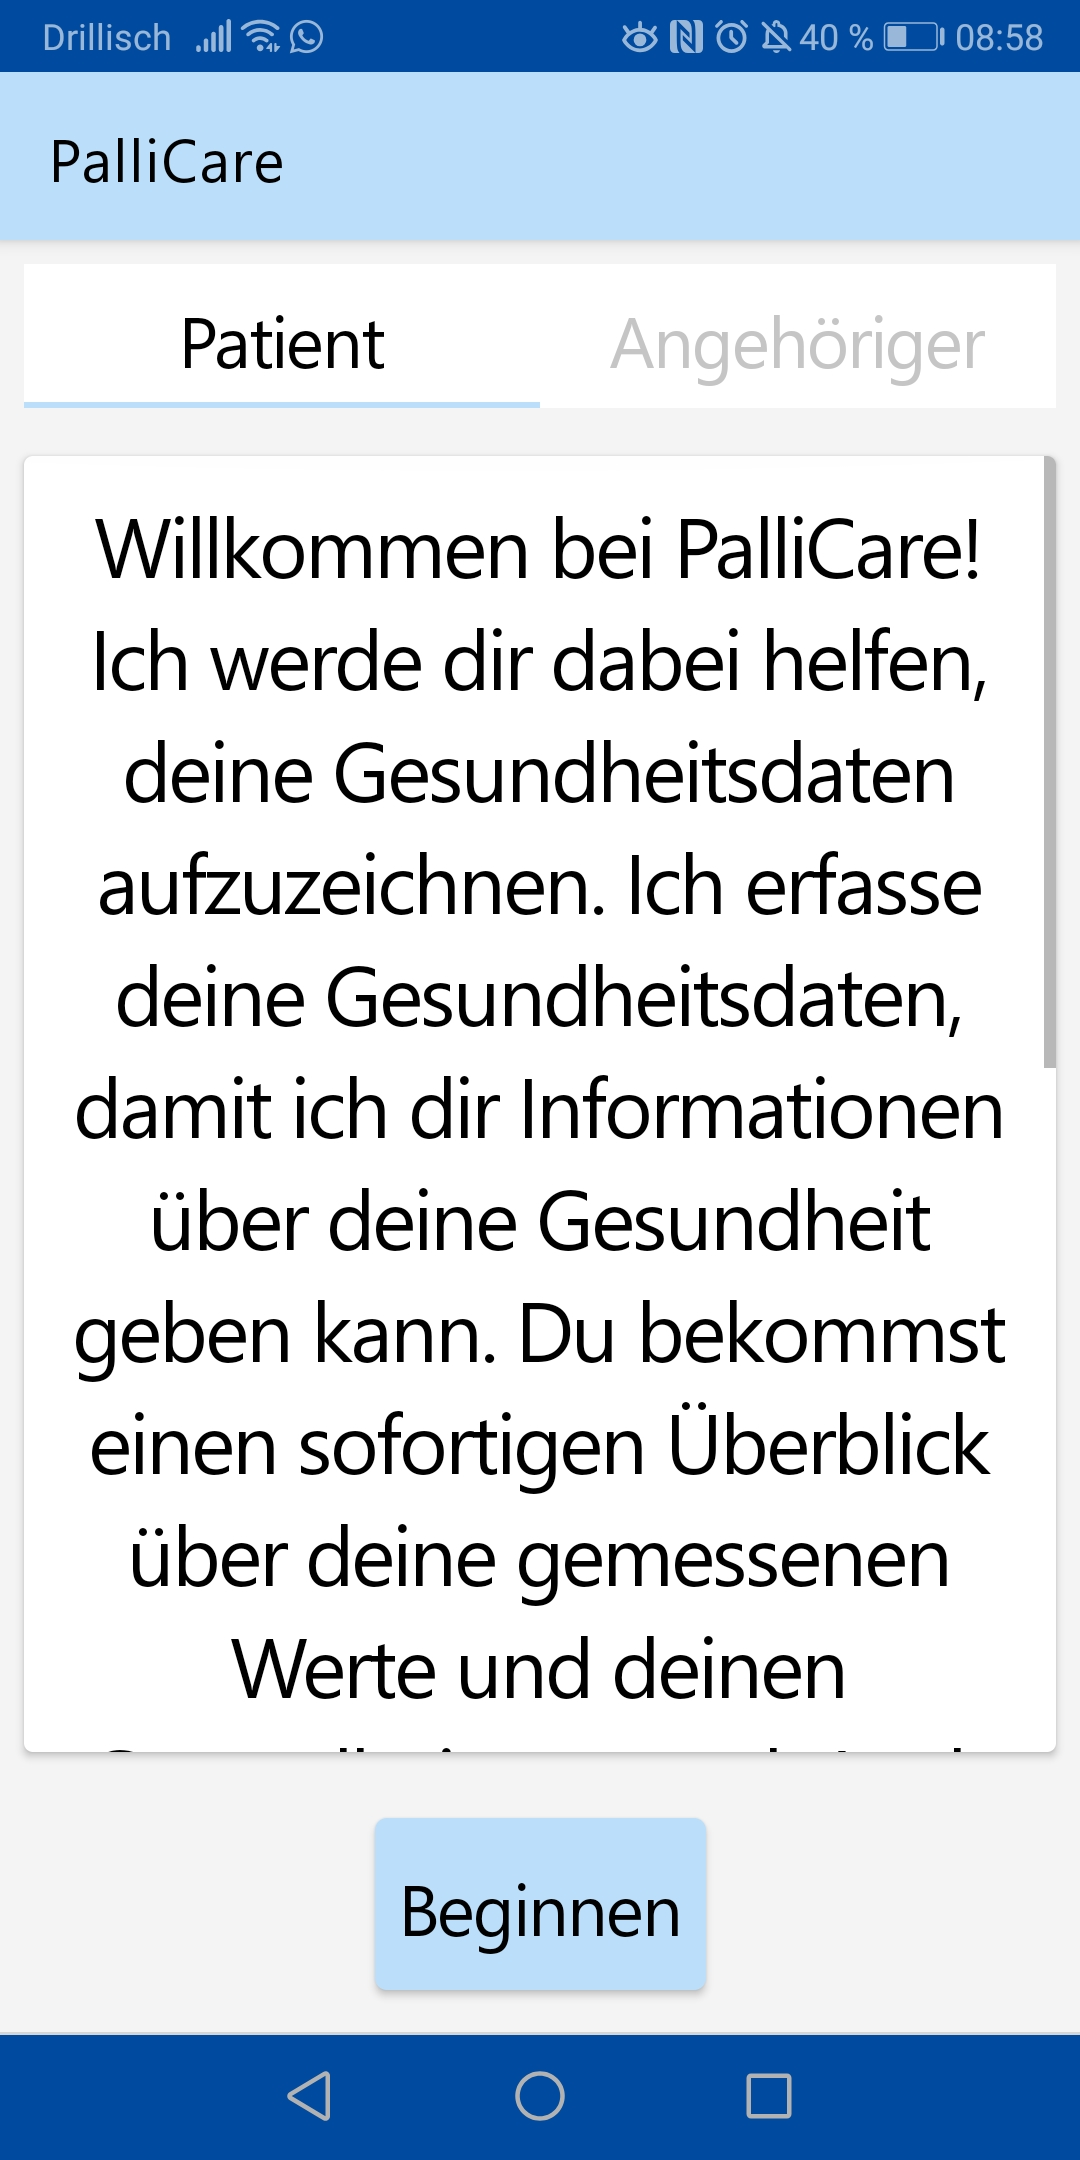
\includegraphics[width=4cm]{figures/welcome_patient.png}
    \caption{Welcome Screen for palliative patients}
    \label{fig:welcome_patient}
\end{figure}
The welcome text for the nok contains the information that the user is a contact and emergency person and that the user has an overview of the patient's data (see Figure \ref{fig:welcome_nok}). 
\newline \newline
\fbox{\parbox{\textwidth}{„Willkommen bei PalliCare! Sie werden eine Kontakt- und Notfallperson für einen Patienten sein. Ich werde die Gesundheitsdaten des Patienten aufzeichnen, damit ich ihm/ihr Informationen über die Gesundheit geben kann. Sie können diese Daten anschauen und somit einen Überblick über den Gesundheitszustand des Patienten bekommen. Im Notfall, falls es dem Patienten nicht gut geht, werden Sie benachrichtigt und somit sofort eingreifen, falls es ihm/ihr nicht gut gehen sollte. Durch Sie wird sich der Patient sicher fühlen und auch Sie werden immer einen Überblick über den Gesundheitszustand des Patienten haben. Lass uns beginnen!“}}
\begin{figure}[H]
    \centering
    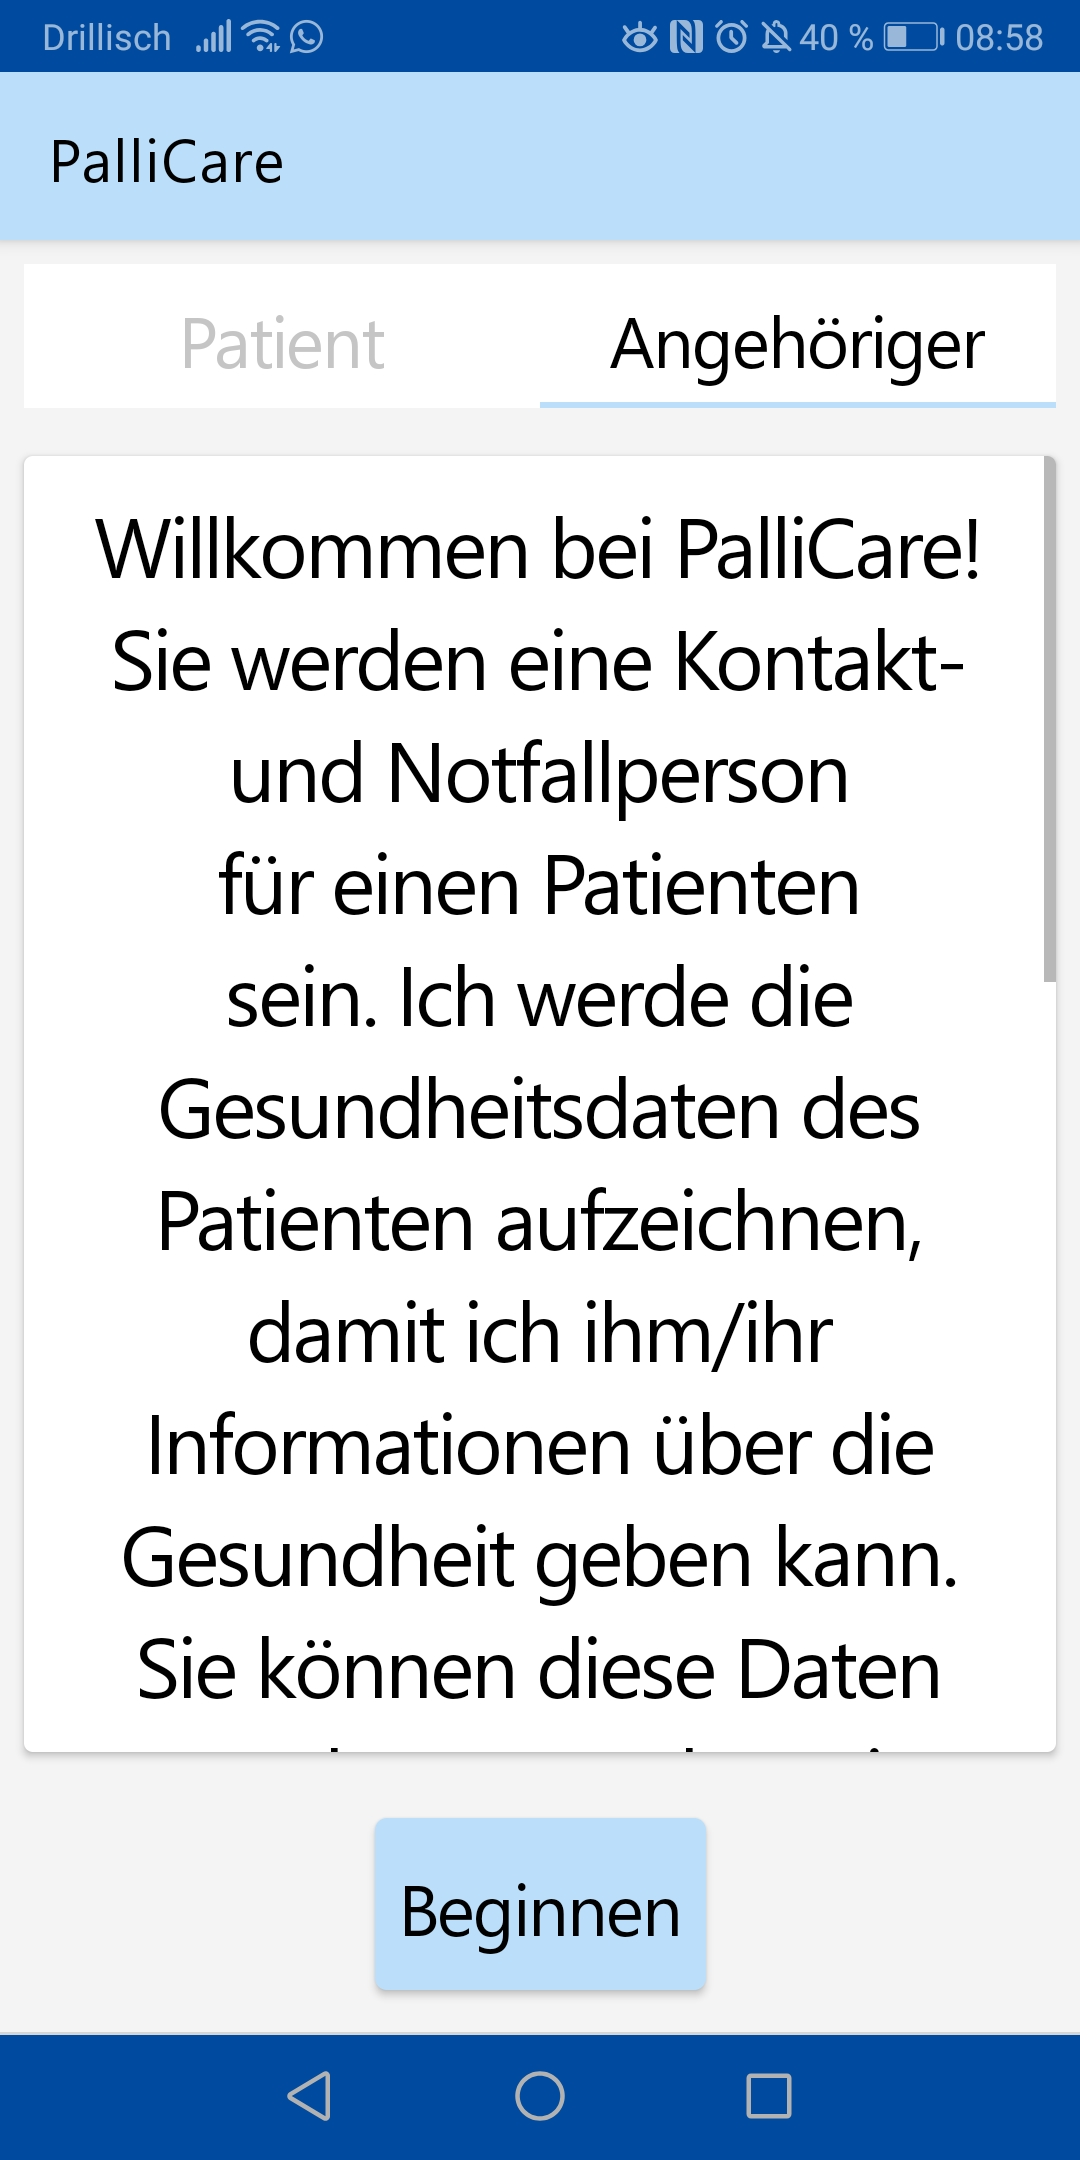
\includegraphics[width=4cm]{figures/welcome_nok.jpg}
    \caption{Welcome Screen for nok}
    \label{fig:welcome_nok}
\end{figure}
After the welcome screen the user has to accept some permissions that are needed for the use of the app. 

First the user must accept the bluetooth permission. This is needed to allow the app to connect to the body scale to record the body weight. This connection also requires access to the location.
\newline \newline
\fbox{\parbox{\textwidth}{„Zur Erfassung Ihrer Gesundheitsdaten wird die Waage mit Ihrem Smartphone über Bluetooth verbunden. Dafür wird der Zugriff auf Ihren Standort benötigt, damit die Verbindung funktionieren kann.“}}
\newline \newline
Afterwards the permission for external and internal storage is required so that the patient's data can be stored on the smartphone.
\newline \newline
\fbox{\parbox{\textwidth}{„Die App erfasst auch Ihre Gesundheitsdaten, damit sie Ihnen Informationen über Ihre Gesundheit geben kann. Zur Speicherung Ihrer Daten benötigen wir Ihre Erlaubnis, dass diese Daten auf Ihrem Handyspeicher gespeichert werden können.“}}
\newline \newline
The last permission is for the emergency button so that the app can make a call. If a patient uses the emergency button, one of the stored emergency contacts is automatically called. 
\newline \newline
\fbox{\parbox{\textwidth}{„Im Folgenden benötigt die App einige Zugriffsberechtigungen. Falls es Ihnen nicht gut gehen sollte, können Sie im Notfall mit Hilfe der App eine Person anrufen, deren Nummer Sie vorher eingespeichert haben. Dafür benötigt die App Ihre Erlaubnis, jemanden anzurufen. Die App verwendet nicht Ihr Telefonbuch.“}}
